
\documentclass[11pt]{beamer}
\usetheme{Frankfurt}
\usecolortheme{seahorse}
\usepackage{multirow}
\usepackage{pifont}
\usepackage{bm}
\usepackage{caption}
%\usepackage{subcaption}
\usepackage{url}


\setbeamertemplate{footline}[frame number]
\setbeamertemplate{itemize items}[triangle]
\setbeamertemplate{frametitle}[default][center]




% Symbols
\newcommand{\ra}{\rightarrow}
\newcommand{\ov}{\overline}
\newcommand{\ur}{\underline}
\newcommand{\pr}{\prime}
\newcommand{\tbf}{\textbf}
\newcommand{\omg}{\Omega}
\newcommand{\mc}{\mathcal}
\newcommand{\lt}{\left}
\newcommand{\rt}{\right}
\newcommand{\mb}{\mathbb}
\newcommand{\imp}{\implies}
\newcommand{\dimp}{\Leftrightarrow}
\newcommand{\wh}{\widehat}
\newcommand{\dg}{\mc{D}}


% Sets
\newcommand{\realset}{\mb{R}}
\newcommand{\comprealset}{\mb{\ov{R}}}
\newcommand{\pint}{\mb{Z}_{> 0}}
\newcommand{\nzrl}{\mb{R}_{\geq 0}}
\newcommand{\prl}{\mb{R}_{>0}}
\newcommand{\rl}{\mb{R}}
\newcommand{\fin}{\forall i\in\{1,...,n\}}
\newcommand{\tup}[1]{\{1,...,#1\}}
\newcommand{\seq}[2]{_{#1=1}^#2}
\newcommand{\mCnn}{\mb{M}_{n\times n}(\mb{C})}
\newcommand{\mCmm}{\mb{M}_{m\times m}(\mb{C})}
\newcommand{\mCpn}{\mb{M}_{p\times n}(\mb{C})}
\newcommand{\mCnm}{\mb{M}_{n\times m}(\mb{C})}
\newcommand{\mRnn}{\mb{M}_{n\times n}(\mb{R})}
\newcommand{\mRpn}{\mb{M}_{p\times n}(\mb{R})}
\newcommand{\mRnm}{\mb{M}_{n\times m}(\mb{R})}
\newcommand{\mRno}{{{\mb{R}}}^n_{\geq 0}}
\newcommand{\mRmo}{{{\mb{R}}}^m_{\geq 0}}
\newcommand{\mRo}{\mb{R}_{\geq 0}}
\newcommand{\mRn}{{\mb{R}}^n}
\newcommand{\mRm}{{\mb{R}}^m}
\newcommand{\mCn}{\mb{C}^n}
\newcommand{\mCm}{\mb{C}^m}
\newcommand{\inv}{\mb{GL}_n(\mb{R})}
\newcommand{\id}[1]{\mb{I}_{#1\times #1}}
\newcommand{\mat}[3]{\mb{M}_{#1\times #2}(\mb{#3})}


% matrix operations
\newcommand{\ColumnJoin}[2]{\left[\begin{array}{l}{#1}\\{#2} \end{array}\right]}
\newcommand{\minaffine}[2]{\Lambda^{\min}\lt(#1,#2\rt)}
\newcommand{\maxaffine}[2]{\Lambda^{\max}\lt(#1,#2\rt)}

% local macros
\DeclareMathOperator{\real}{\operatorname{Re}}
\newcommand{\CZ}{\lt(V,c,s\rt)}
\newcommand{\GCZ}{\gcz{V}{c}{s}{W}{l}{u}}
\newcommand{\cz}[3]{\mc{C}\lt(#1,#2,#3\rt)}
\newcommand{\CZO}{\lt(V,0,s\rt)}
\newcommand{\czo}[2]{\mc{Z}\lt(#1,0,#2\rt)}
\newcommand{\trj}[2]{{\bf #1}(#2)}
\newcommand{\IncTcz}[6]{\mc{T}\lt(#1,#2,#3,#4,#5,#6\rt)}
\newcommand{\IncGcz}[6]{\mc{G}\lt(#1,#2,#3,#4,#5,#6\rt)}
\newcommand{\Ptope}[3]{\mc{P}\left(#1,#2,#3\right)}
\newcommand{\gcz}[6]{\mathcal{Z}\lt(#1,#2,#3,#4,#5,#6\rt)}
\newcommand{\sptope}[3]{\mathcal{P}\lt(#1,#2,#3\rt)}
\newcommand{\system}{\mb{H}}
\newcommand{\locationset}{Q}
\newcommand{\edgeset}{E}
\newcommand{\stay}{\gamma}
\newcommand{\linearmapset}{\mc{A}}
\newcommand{\inputset}{U}
\newcommand{\initialset}{\Omega}
\newcommand{\edge}{\sigma}
\newcommand{\loc}{q}
\newcommand{\map}{\linearmapset}
\newcommand{\inp}{\inputset}
\newcommand{\ptemplate}{\mc{K}}
\newcommand{\systrj}[2]{\lt({\bf #1},{\bf #2}\rt)}
\newcommand{\wholenums}{\mb{Z}_\geq 0}
\newcommand{\preloc}[1]{#1_{1}}
\newcommand{\postloc}[1]{#1_{2}}
\newcommand{\upperedgebound}[1]{#1^+}
\newcommand{\loweredgebound}[1]{#1^-}
\newcommand{\reset}[1]{#1_r}
\newcommand{\locationtransition}[1]{R_{#1}}
\newcommand{\edgetransition}[1]{R_{#1}}
\newcommand{\staysptope}[1]{\sptope{\ptemplate\lt(#1\rt)}{\stay^-\lt(#1\rt)}{\stay^+\lt(#1\rt)}}
\newcommand{\guardsptope}[1]{\sptope{\ptemplate\lt(\preloc{#1}\rt)}{\max\lt(\loweredgebound{#1},\stay^-\lt(\preloc{#1}\rt)\rt)}{\min\lt(\upperedgebound{#1},\stay^+\lt(\preloc{#1}\rt) \rt)}}
\newcommand{\hybridset}{\Gamma}
\newcommand{\transfer}[4]{#1#4 = #2\dg\lt(#3\rt)}
\newcommand{\centertransfer}[4]{#1#4 = #3-#2}
\newcommand{\scalebound}[5]{\max_{i=1}^{#4}\lt(\lt(\sum_{j=1}^{#5}\lt|#1\rt|_j\rt)-#3_i+#2_i\rt)}
\newcommand{\pseudoinverse}[1]{#1\lt(#1#1^T\rt)^{-1}}


\title{Complex Zonotopes for Safety Verification of Discrete Time Affine Hybrid Systems}
\setbeamercolor{author}{fg=blue}
\author[shortname]{{  \bf \hspace{-1em} Arvind\ Adimoolam~\inst{1}\hspace{1em} Thao\ Dang~\inst{2}}}
\setbeamercolor{institute}{fg=blue}
\institute{{\bf 
\inst{1,2} VERIMAG/ \inst{2}CNRS}\\~Grenoble,France
\begin{figure}
\center
\hspace{2em}
\includegraphics[scale=0.2]{figures/LogoVERIMAG.png}
\end{figure}
}

\date{}

\begin{document}
\maketitle

\begin{frame}{Discrete time dynamical system}
%
Models evolution of system state measured at discrete instants of time.
\begin{figure}
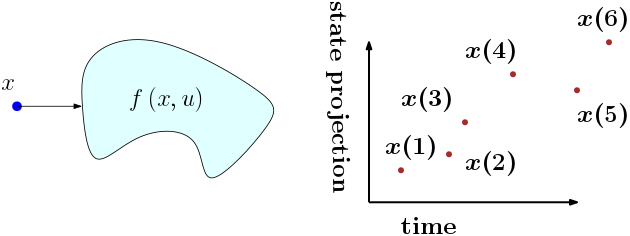
\includegraphics[scale=0.4]{figures/dynamical-system.png}
\end{figure}
%
\begin{itemize}
\item {\color{blue} Discrete time linear system}:\\
Let {\color{purple} $\bm{x}(t)$} denote {\color{blue} state of system}
at time $t$, {\color{purple} $\bm{u}(t)$} denote {\color{blue} input},
which {\color{blue} belongs} to a set {\color{purple}
$U\subseteq \mathbb{R}^p$}.
%
{\color{purple}
\[
\bm{x}(t+1)=A\bm{x}(t)+\bm{u}.
\]
}
\end{itemize}
\end{frame}

\begin{frame}{Discrete time affine hybrid system}

{\color{blue} Collection of linear systems} with {\color{blue} conditions for switching}.
%
\begin{figure}
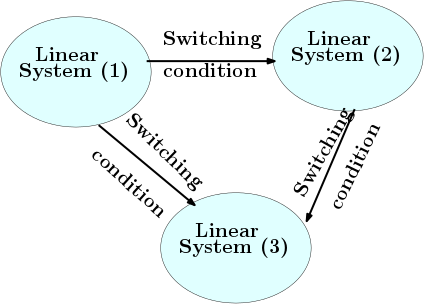
\includegraphics[scale=0.5]{figures/affine-hybrid.png}
\end{figure}
%
\end{frame}



\begin{frame}{Safety verification}

{\color{violet} Verify:} {\color{blue} Set of all reachable states} is {\color{blue} contained inside a safe set.}

{\color{purple} \[ R_t(X_0)  = A^tX_0\oplus A^{t-1}U\oplus A^{t-2}U\oplus ...\oplus AU+U\].}\vspace{-2em}

{\color{purple} \[\text{Reachable set} = \bigcup_{t=0}^\infty R_t(X_0)\]}.
%
\begin{figure}
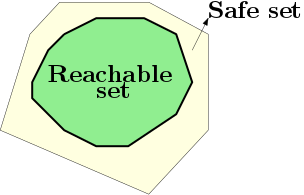
\includegraphics[scale=0.5]{figures/safety.png}
\end{figure}
%
\end{frame}

\begin{frame}{Over-approximating reach set using a set representation}
\begin{itemize}
\item {\color{purple} Exact reachable set} can be {\color{purple} computationally expensive} to {\color{purple} represent}.
\end{itemize}
%
Instead, {\color{blue}compute} a {\color{blue} concise set
representation} that is {\color{blue} over-approximation} of exact
reach set.
%
\begin{alertblock}{}
{\bf Set representation}: {\color{blue} Data structure} used to denote
a {\color{blue} geometric shape}.  Eg. {\color{purple} Polytope}: $\lt(T,d\rt): Tx\leq d$,
{\color{purple} Ellipsoid}: $\lt(P\rt): x^TPx\leq 1$.
\end{alertblock}
%
\begin{figure}
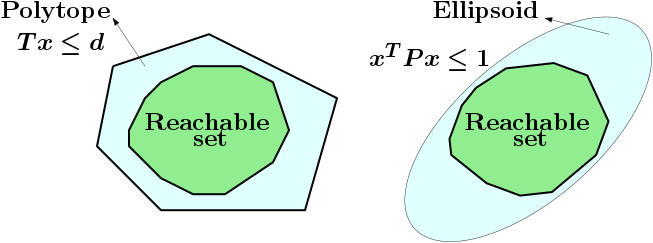
\includegraphics[scale=0.35]{figures/set-representation.png}
\end{figure}
%
\end{frame}


\begin{frame}{Features of good set representation}
\begin{enumerate}
\item
\begin{minipage}{0.4\textwidth}
{\color{blue} Accuracy} of approximating reach set.
\end{minipage}
%
\hfill\hfill
%
\begin{minipage}{0.5\textwidth}
\begin{figure}
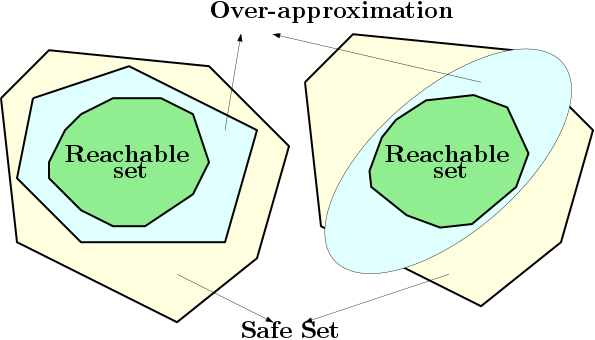
\includegraphics[scale=0.3]{figures/accuracy-approximation.png}
\end{figure}
\end{minipage}
%
\pause
%
\item Efficiently compute {\color{blue} positive invariants}.
{\color{purple} Positive invariance $\Rightarrow$} Proof of
{\color{purple} valid over-approximation} for \underline{unbounded time}.
%
\begin{figure}
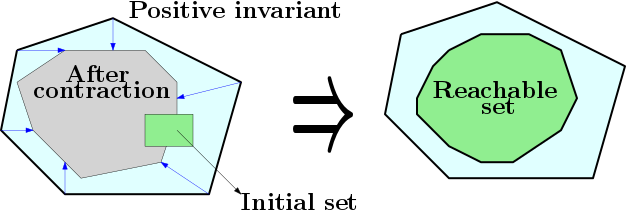
\includegraphics[scale=0.35]{figures/positive-invariant.png}
\end{figure}
%
\end{enumerate}
\end{frame}

\begin{frame}{Simple Zonotope}
%
\begin{itemize}
\item Let {\color{purple} $W\in\mat{n}{k}{\reals}$} called {\color{blue}
generator matrix}, {\color{purple} $l,u\in\reals^k:~l\leq u$} called
{\color{blue} upper and lower coefficient bounds}.
%
\[
{\color{purple}
\rztope{W}{l}{u}=\set{V\zeta:\zeta\in\reals^k,~l\leq \zeta\leq u}
}
\]
\item Geometrically, {\color{blue} Minkowski sum of line segments}.
\end{itemize}
\begin{minipage}{0.65\textwidth}
\begin{figure}
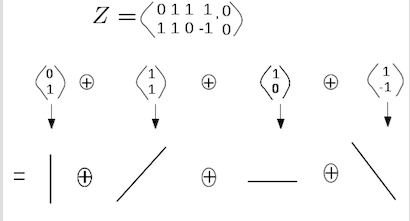
\includegraphics[trim={2mm 0 2mm 1.5cm},clip,scale=0.45]{figures/rz1.png}
\end{figure}
\end{minipage}
%
\begin{minipage}{0.25\textwidth}
\begin{figure}
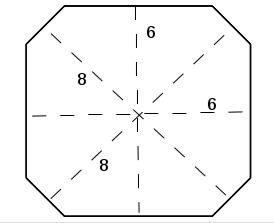
\includegraphics[trim={0 3cm 0 0},scale=0.4]{figures/rz2.png}
\end{figure}
\end{minipage}
%
{\small
\begin{thebibliography}{1}

\bibitem{girard2005reachability}
Antoine Girard.
\newblock Reachability of uncertain linear systems using zonotopes.
\newblock In {\em HSCC}, volume~5, pages 291--305. Springer, 2005.

\end{thebibliography}
}
\end{frame}


\begin{frame}{Advantage of Simple zonotope over other representations}
Consider {\color{purple} box disturbance input} and {\color{purple}
box initial set}
%
{\color{purple} \[ R_t(X_0)  = A^tX_0\oplus A^{t-1}U\oplus
A^{t-2}U\oplus ...\oplus AU+U\].}\vspace{-2em}
%
\begin{itemize}
\item
\begin{enumerate}
\item   {\color{blue} Linear transformation} and
{\color{blue} Minkowski sum} are {\color{blue} closed operations on zonotopes} and
{\color{blue} representation size is same}.
\item {\color{blue} Using zonotope}, representing $R_t(X_0)$ requires {\color{blue} $tn$} vectors.
\end{enumerate}
\item {\color{purple} Using polytope}, respresenting $R_t(X_0)$
requires {\color{purple}$t\choose n$: exponential} no. generators.
\item {\color{purple} Ellipsoids have smooth boundary}, tend to have
{\color{purple} large
over-approximation error}.
\end{itemize}
%
{\color{black} Accurate bounded time computation} $\Rightarrow$
{\color{black} Reduces
over-approximation error in unbounded time reach set approximation}.
\end{frame}

%
\begin{frame}{Positive invariant zonotopes based on eigenvectors}
\begin{itemize}
\item {\color{blue}Zonotopes} with {\color{blue} stable eigenvectors as generators} are
{\color{blue} invariant} w.r.t linear transformation.
\item Let {\color{blue} $A$} be a {\color{blue}stable matrix} with
{\color{blue}$e$: vector of real eigenvectors} and {\color{blue}$\mu$:
vector of real eigenvalues}.  Then,
%
{\color{purple}
\begin{align*}
 A\rztope{[e_1,...,e_n]}{l}{u}   = \rztope{[e_1,...,e_n]}{\diagonal{\absolute{\mu}}l}{\diagonal{\absolute{\mu}}u}
\end{align*}
}
%
\begin{figure}
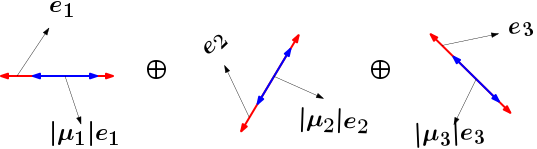
\includegraphics[scale=0.5]{figures/contraction-zonotope.png}
\end{figure}
%
\end{itemize}
\end{frame}

\begin{frame}{Complex zonotope}

\begin{alertblock}{Problem}
{\color{purple} How to incorporate} {\color{blue} complex-valued eigenvectors} in
{\color{purple} generators to define} {\color{blue} positive invariants ?}
\end{alertblock}
%
\pause
%
\begin{block}{Answer: Complex zonotope}
{\color{blue} Linear combination} of
{\color{blue} complex-valued eigenvectors} such that {\color{blue}
complex combining coefficients} are \underline{{\color{purple} bounded in absolute
values (quadratic constraint)}}.
\end{block}
%
\begin{block}{}
Let \eqncol{$\ptemp\in\mat{n}{m}{\compnums}$} called \textcol{template},
\eqncol{$\cen\in\compnums^n$} called \textcol{center} and \eqncol{$\sfact\in\reals_{\geq 0}^m$}
called \textcol{scaling factors}.
%
{\color{black}
\[
\bm{
\tcztope{V}{c}{s}=\set{V\zeta+c:~\zeta\in\compnums^m,~\absolute{\zeta}\leq
s}
}
\]
}
\end{block}
%
\end{frame}

\begin{frame}{Geometric visualization: Complex zonotope}
\begin{itemize}
\item Represent {\color{blue} wider class of sets} than {\color{purple} real zonotopes}.
\item {\color{blue} Minkowski sum} of {\color{purple}line segments}
and also {\color{blue} some ellipsoids}.
\item Can represent some {\color{blue} non-polyhedral} sets in
addition to {\color{purple} polytopic real zonotopes}.
\end{itemize}
%
\begin{figure}
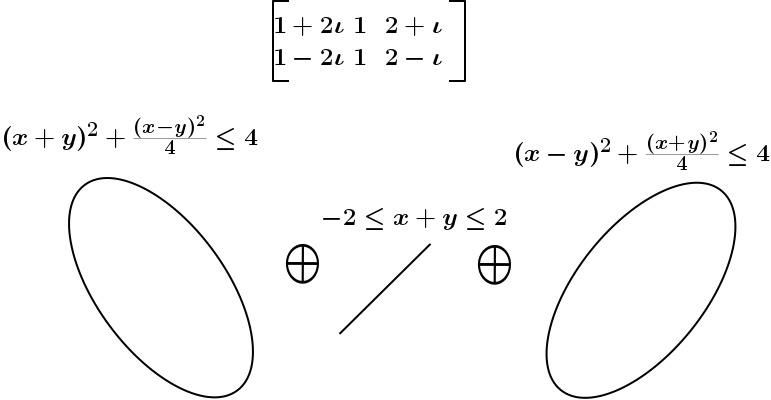
\includegraphics[scale=0.45]{figures/complex-zonotope.png}
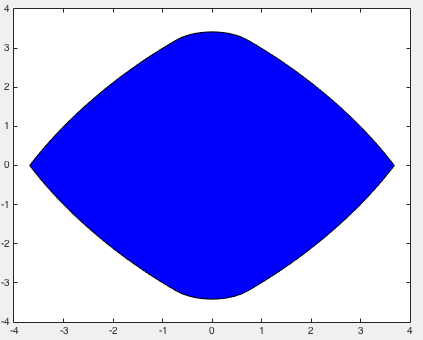
\includegraphics[scale=0.3]{figures/CZhull.png}
\end{figure}
%
\end{frame}

\begin{frame}{Advantage: Complex eigenstructure based Contraction}
Consider {\color{blue} matrix $A\in\mat{n}{n}{R}$} with {\color{blue} eigenvectors $e_1,...,e_n$}
and {\color{blue} $\mu$: vector of eigenvalues}.
%
{\color{purple}
\begin{align*}
 A\tcztope{[e_1,...,e_n]}{0}{\sfact}   = \tcztope{[e_1,...,e_n]}{0}{\diagonal{\absolute{\mu}}\sfact}
\end{align*}
}
%
\center{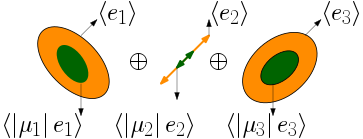
\includegraphics[scale=0.6      ]{figures/ContractionCZ.png}}
\end{frame}


\begin{frame}{Ambiguity in over-approximation using
limited generators}
\begin{block}{Need to fix maximum number of generators}
{\color{purple} Complexity} of representing of {\color{purple}
reach set after large time} reach set is {\color{purple} high}.  But we
{\color{blue} can only use limited number of generators} and compute
over-approximation depending on {\color{purple} computation resources}.
\end{block}
%
\begin{block}{Ambiguity in over-approximation}
For a {\color{blue} fixed number of generators}, there is {\color{purple} no smallest zonotope}
approximating a given set.
\end{block}
\end{frame}

\begin{frame}{Our approach}
We have to solve:
{\color{purple}
\begin{align*}
& A\tcztope{V}{c}{s}\oplus U\subseteq \tcztope{V}{c}{s}\\
& \tcztope{V}{c}{s}\subseteq S~\text{(safe set)}\\
& X_0~\text{(Initial set)}~\subseteq \tcztope{V}{c}{s}
\end{align*}
}
%
\begin{block}{Solution: Derive convex relaxation}
For a {\color{purple} fixed template ($V$)}, we derive
{\color{blue} convex constraints on
$c$ and $s$} as {\color{blue} sufficient conditions} for above.
\end{block}
%
\begin{thebibliography}{1}

\bibitem{adimoolam2017augmented}
{\small
Arvind Adimoolam and Thao Dang.
\newblock Augmented complex zonotopes for computing invariants of affine hybrid
  systems.
\newblock In {\em International Conference on Formal Modeling and Analysis of
  Timed Systems}, pages 97--115. Springer, 2017.
  }
\end{thebibliography}

\end{frame}

\begin{frame}{Example 1: NXT-Lego Robot model}
\eqncol{Benchmark example} published in \eqncol{ARCH 2014~\cite{heinz2014benchmark}} \textcol{(Heinz, Oehlerking and Woehrle.)}

\begin{minipage}{0.3\textwidth}
\begin{figure}
\centering
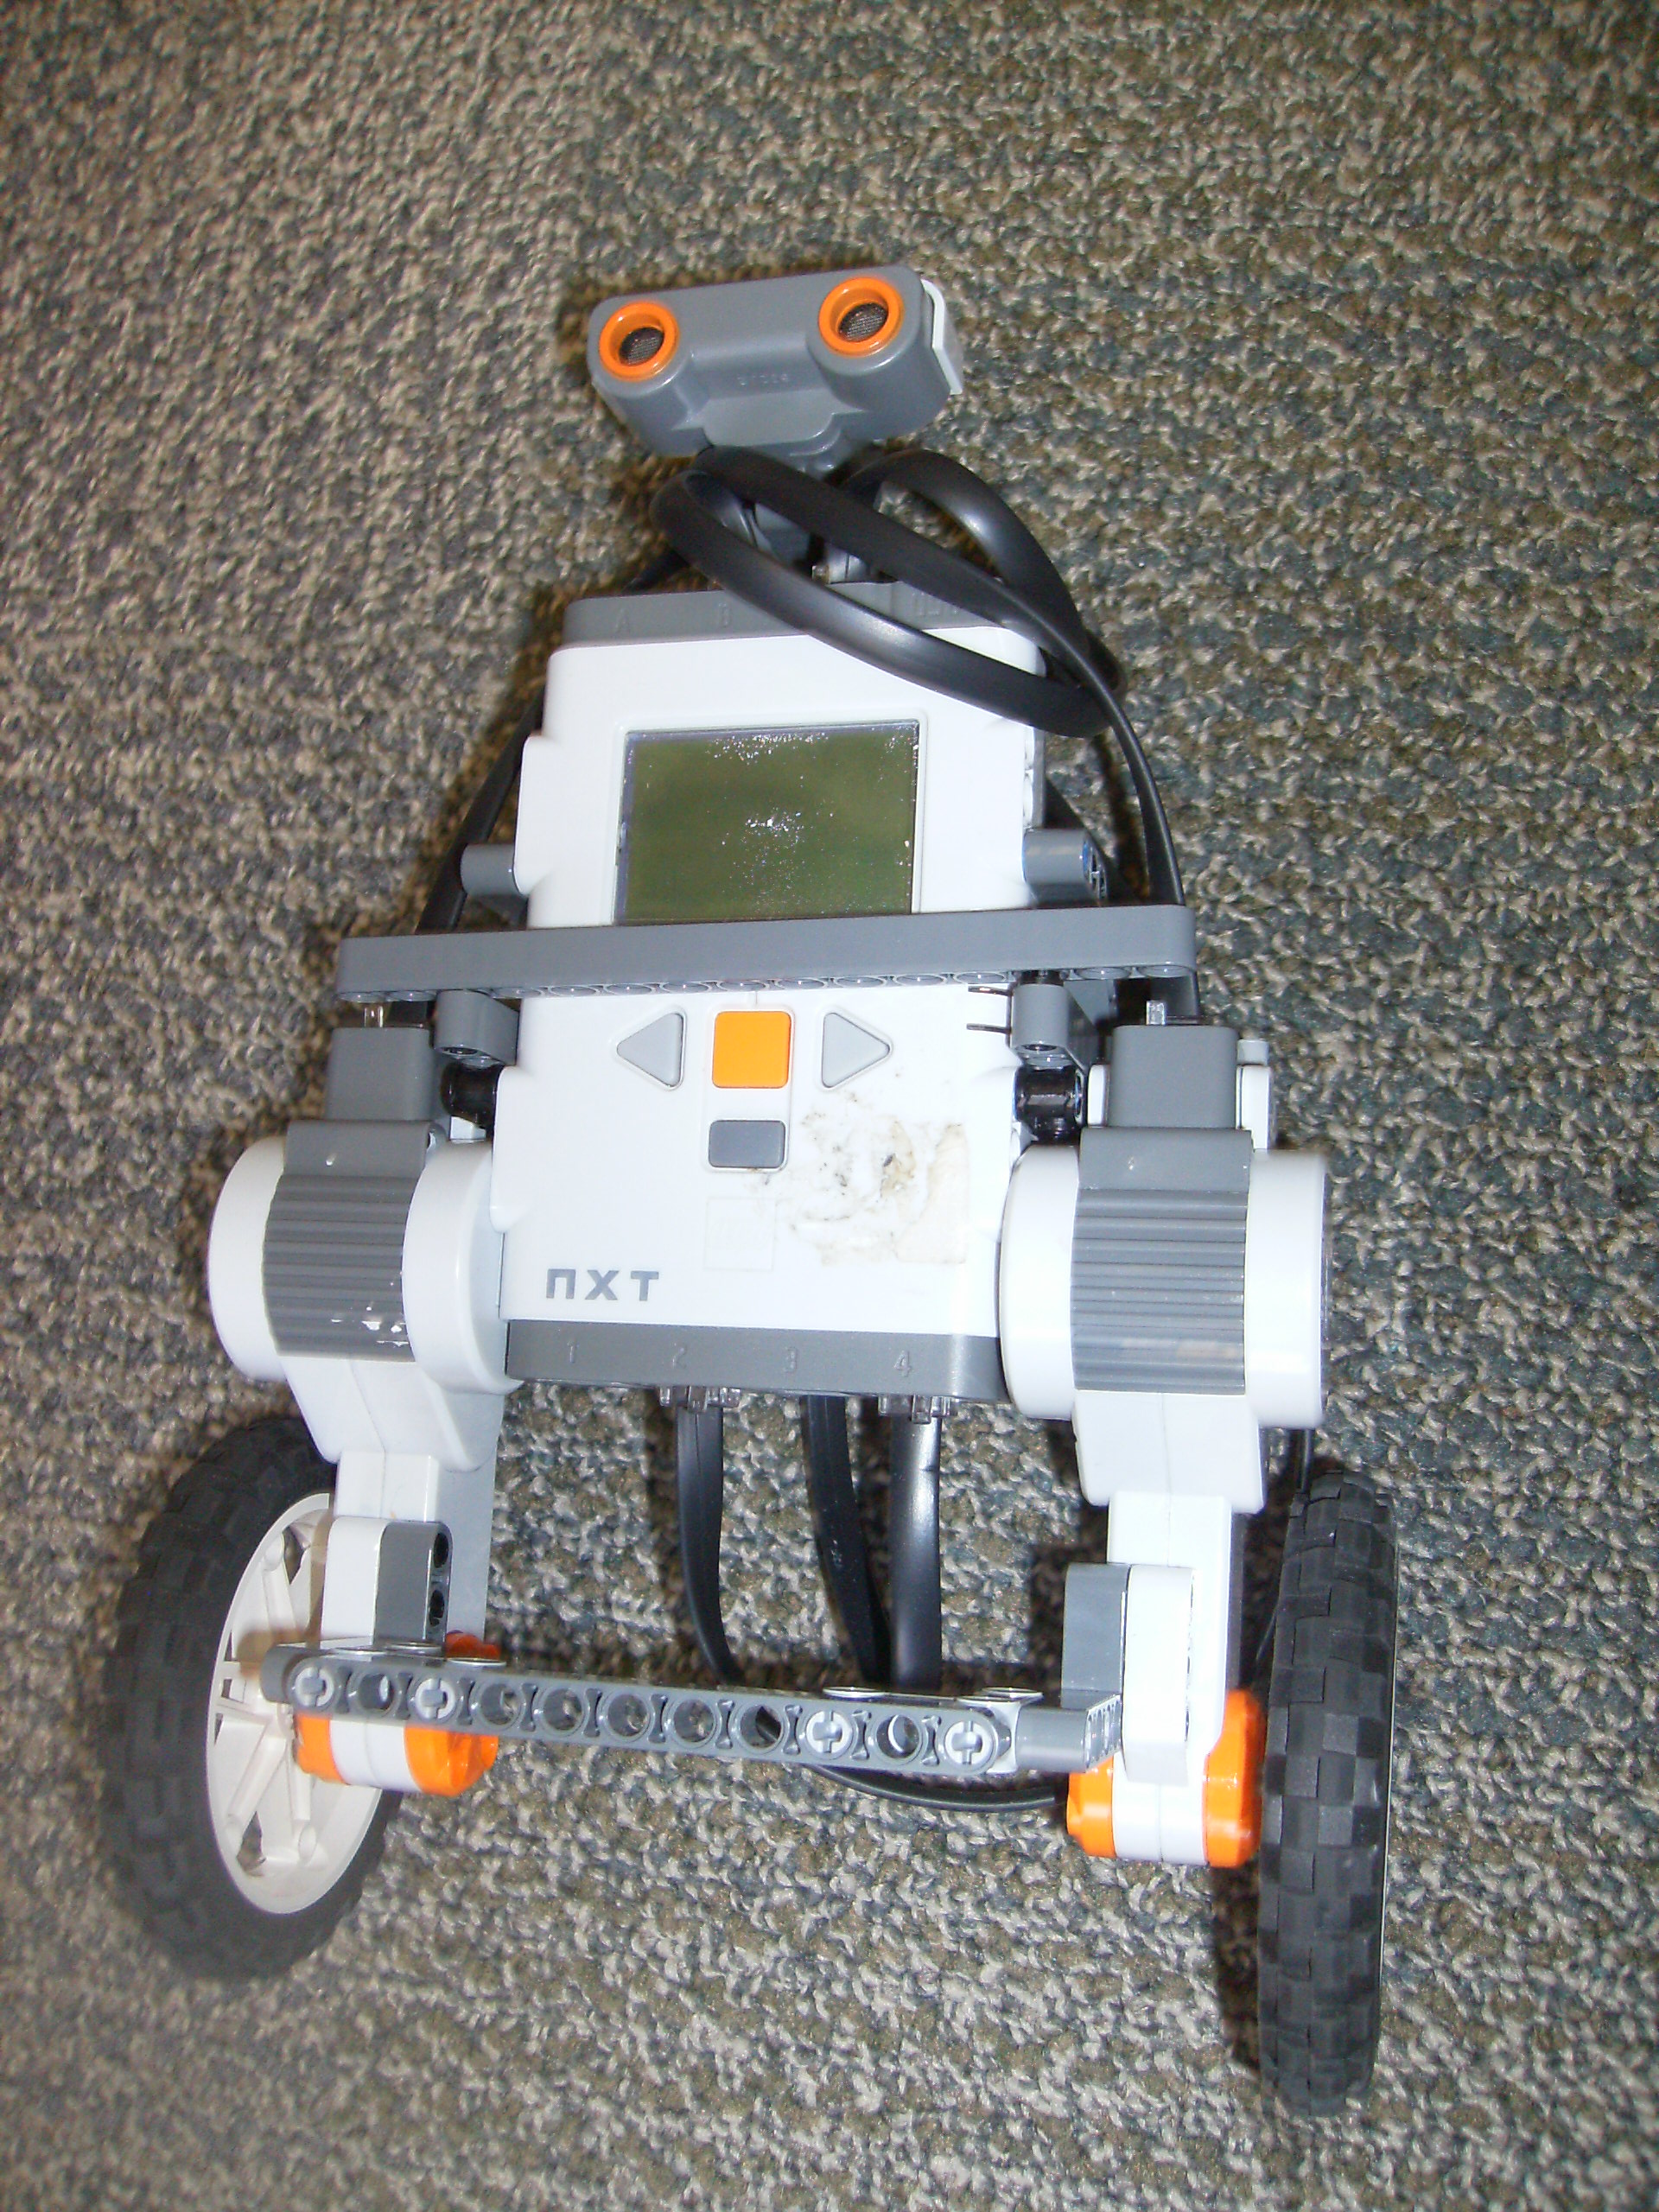
\includegraphics[scale=0.09]{fig/NXT-lego.JPG}
\end{figure}
\end{minipage}
\begin{minipage}{0.6\textwidth}
{\footnotesize Lego NXT self-balancing robot by\\ Medelen8/CC-BY-SA-3.0}
\begin{itemize}
\item \textcol{Sampled data Networked Control System}: Controller input to Plant sampled at discrete time instants.
\item Input from controller has \textcol{saturation} on {\color{violet} 2 controller inputs}: \textcol{Hybrid behavior}.
\end{itemize}
\end{minipage}

%% \begin{block}{}
%% $
%% \lt[\begin{array}{cc}\trj{x}{t+1} &
%%     \trj{y}{t+1}\end{array}\rt]^T=F_1\trj{x}{t}+F_2sat\lt(\trj{y}{t}\rt)+F_3\trj{u}{t}$\\
%% \textcol{Saturated}: $sat\lt(y_i\rt) = max\lt(-\delta
%% d_p,min\lt(y_i,\delta d_p\rt)\rt),~\forall i\in\{1,2\}$, where $\delta=100$
%% and $d_p=0.0807$. \textcol{Unsaturated}: $sat\lt(y_i\rt) = y_i$
%% \end{block}
\end{frame}


\begin{frame}{Verification challege: NXT-Lego Robot model}
\begin{alertblock}{Task}
Find/Verify bounds on \textcol{body pitch angle}.
\end{alertblock}
%
\eqncol{After transformation to decouple unbounded directions, we
obtained}\\
%
\begin{block}{Complexity}
\begin{itemize}
\item \eqncol{Saturated}: \textcol{9 dimensional, 1 location, 9 edges.}
\item \eqncol{Unsaturated}: \textcol{9 dimensional linear system.}
\end{itemize}
\end{block}
%
\end{frame}

\begin{frame}{Experimental settings}
%
\begin{itemize}
\item \eqncol{Primary template:}  (Complex) \textcol{Eigenvectors} of linear maps and their products,
 \textcol{Orthonormal
vectors} to guarding hyperplane normals.  For
the linear system, it consists of the eigenvectors of the linear map,
the \textcol{uncertain input set template} and its multiplication by the linear matrix
(related to affine map) and square of the linear matrix. 
\item \eqncol{SpaceEx settings:}  \textcol{Octagon template} and a
template with \textcol{$400$ uniformly sampled support vectors}.
\end{itemize}
%
\end{frame}


\begin{frame}{Results: NXT-Lego Robot model}
\center{{\eqncol{\small{\footnotesize UB: $>$1000, ~~NT: Not terminating in more than 180s, \newline
  n/a: Not applicable/not available, ~~ACZ: Augmented complex
  zonotope.}}}}
{\color{black}
\begin{minipage}{0.48\textwidth}
\begin{table}
\centering
\resizebox{0.5\textheight}{0.35\textwidth}{
\begin{tabular}{|l|c|c|c|}
\hline
\multicolumn{2}{|c|}{\multirow{2}{*}{Method}} &
\multirow{2}{*}{$\lt|\psi\rt|\leq$} & Comp.\\
\multicolumn{2}{|c|}{} & & time (s)\\
\hline
\multirow{4}{*}{SpaceEx} & octagon & \multirow{2}{*}{UB} & \multirow{2}{*}{NT}\\
& template & & \\
\cline{2-4}
& 400 support & \multirow{2}{*}{UB} & \multirow{2}{*}{NT}\\
& vectors & &\\
\hline
\multicolumn{2}{|c|}{\multirow{2}{*}{Suggested in~\cite{heinz2014benchmark}}} &
\multirow{2}{*}{$1.39$} & \multirow{2}{*}{n/a}\\
\multicolumn{2}{|c|}{} & &\\
\hline
\multicolumn{2}{|c|}{\multirow{2}{*}{ACZ invariant}} & \multirow{2}{*}{$1.29$} &
\multirow{2}{*}{$4$}\\
\multicolumn{2}{|c|}{} & & \\
\hline
\end{tabular}
}
\caption*{{\footnotesize Unsaturated robot model: results}}
\end{table}
\end{minipage}
\begin{minipage}{0.48\textwidth}
\begin{table}
\centering
\resizebox{0.5\textheight}{0.35\textwidth}{
\begin{tabular}{|l|c|c|c|}
\hline
\multicolumn{2}{|c|}{\multirow{2}{*}{Method}} &
\multirow{2}{*}{$\lt|\psi\rt|\leq$} & Comp.\\
\multicolumn{2}{|c|}{} & & time (s)\\
\hline
\multirow{4}{*}{SpaceEx} & octagon & \multirow{2}{*}{UB} &
\multirow{2}{*}{NT}\\
& template & & \\
\cline{2-4}
& 400 support & \multirow{2}{*}{UB} & \multirow{2}{*}{NT}\\
& vectors & & \\
\hline
\multicolumn{2}{|c|}{\multirow{2}{*}{Suggested in~\cite{heinz2014benchmark}}} &
$1.571-\epsilon:$ & \multirow{2}{*}{n/a}\\
\multicolumn{2}{|c|}{} & $\epsilon>0$ &\\
\hline
\multicolumn{2}{|c|}{\multirow{2}{*}{ACZ invariant}} & \multirow{2}{*}{$1.13$} &
\multirow{2}{*}{45}\\
\multicolumn{2}{|c|}{} & &\\
\hline
\end{tabular}
}
\caption*{{\footnotesize Saturated robot model: results}}
\end{table}
\end{minipage}
}
\vspace{-2em}
{\small
\begin{alertblock}{Remarks}
\begin{itemize}
\item Model has \textcol{complex eigenstructure}, some eigenvalues have \textcol{magnitude close to 1}.
\item Since \textcol{Complex Zonotope uses complex eigenstructure}, where as \textcol{Polytope (SpaceEx)} \eqncol{can not use complex eigenstructure}.
\end{itemize}
\end{alertblock}
}
\end{frame}

\begin{frame}{Example 2: Perturbed double integrator}
\begin{itemize}
\item Example from \textcol{Rakovic et. al.-CDC 2004}~\cite{rakovic2004computation}.
\item \textcol{Piecewise affine with 2 dimensional additive disturbance input}, \eqncol{Four different Affine
dynamics} in \eqncol{Four different polytopic regions} of space.
\item Model complexity: \textcol{2 dimensions, 4 locations and 12 edges.}
\end{itemize}
\begin{alertblock}{Challenge}
\begin{enumerate}
\item Verify \textcol{smallest (possible) bounds} on the \textcol{two state space co-ordinates}.
\item Compute a \textcol{large set} of \textcol{safe initial conditions}.
\end{enumerate}
\end{alertblock}
\pause
\begin{exampleblock}{Experimental settings}
\begin{itemize}
\item  {\bf Primary template}: \textcol{Complex eigenvectors} of all linear matrices of the \textcol{affine maps and
their binary products}. 
\item  {\bf SpaceEx tool}: \eqncol{Two
different templates}: \textcol{Octagon} template and a template with \textcol{100
uniformly sampled support vectors}.
\end{itemize}
\end{exampleblock}
\end{frame}

\begin{frame}{Experimental results: PDI}
\begin{table}
\begin{minipage}{\textwidth}
\center
\caption*{Small invariant computation}
{\small
\begin{tabular}{|l|c|c|c|c|}
\hline
\multicolumn{2}{|c|}{\multirow{2}{*}{Method}} &
\multirow{2}{*}{$\lt|x_1\rt|\leq$} & \multirow{2}{*}{$\lt|x_2\rt|\leq$} & Comp.\\
\multicolumn{2}{|c|}{} & & & time (s) \\
\hline
\multirow{4}{*}{SpaceEx} & octagon & \multirow{2}{*}{0.38} &
\multirow{2}{*}{0.43} & \multirow{2}{*}{1.7}\\
& template & & &\\
\cline{2-5}
& 100 support & \multirow{2}{*}{0.38} & \multirow{2}{*}{0.43} & \multirow{2}{*}{23.6}\\
& vectors & & &\\
\hline
\multicolumn{2}{|c|}{\multirow{2}{*}{ACZ invariant}} &
\multirow{2}{*}{0.38} & \multirow{2}{*}{0.36} & 
\multirow{2}{*}{5.1}\\
\multicolumn{2}{|c|}{} & & &\\
\hline
\end{tabular}
}
\end{minipage}
\hspace{4em}
\begin{minipage}{\textwidth}
\center
{\small
\caption*{Large invariant computation}
\begin{tabular}{|c|c|}
\hline
\multirow{2}{*}{Method} & Comp.\\
& time (s)\\
\hline
\multirow{2}{*}{MPT tool~\cite{rakovic2004computation}} & \multirow{2}{*}{107}\\
& \\
\hline
\multirow{2}{*}{ACZ} & \multirow{2}{*}{12}\\
& \\
\hline
\end{tabular}
}
\end{minipage}
\end{table}
\end{frame}

\begin{frame}{Example 3: Networked vehicle platoon}
\begin{figure}
\caption*{\small Benchmark {\color{blue}  2014 ARCH Workshop}: \eqncol{Makhlouf and Kowalewski~\cite{makhlouf2014networked}}}
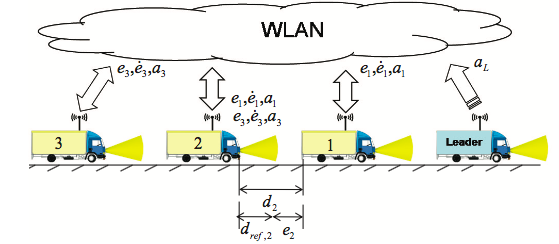
\includegraphics[scale=0.4]{fig/VehiclePlatoon.png}\\
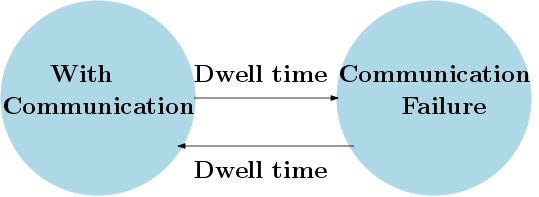
\includegraphics[scale=0.4]{fig/networked-platoon-model.png}
\end{figure}
\end{frame}

\begin{frame}{Verification challenge: Networked platoon}
\begin{alertblock}{Task}
\begin{itemize}
\item Find \textcol{minimum (possible) reference distances between vehicles} such that \eqncol{vehicles do not collide}.
\item Equivalent to finding \textcol{ upper bounds on $-e_1, -e_2$ and $-e_3$}.
\end{itemize}
\end{alertblock}
%
\begin{exampleblock}{Two cases}
\begin{enumerate}
\item \textcol{Slow switching}: \eqncol{Minimum dwell time 20 s}. {\color{violet} 9 dimensional, 2 locations, 4 edges}.
\item \textcol{Fast switching}: \eqncol{Integer dwell times}. {\color{violet} 9 dimensional, 2 locations, 2 edges}.
\end{enumerate}
\end{exampleblock}
\end{frame}

\begin{frame}{Expermimental results: Networked Platoon}
\begin{table}
\resizebox{1.1\textwidth}{!}{\hspace{-3em}
\begin{tabular}{|l|c|c|c|c|c|c|c|c|c|}
\hline
\multicolumn{2}{|c|}{\multirow{4}{*}{Method}} & \multicolumn{4}{|c|}{\multirow{2}{*}{Slow switching}} & \multicolumn{4}{|c|}{\multirow{2}{*}{Fast switching}}\\
\multicolumn{2}{|c|}{} & \multicolumn{4}{|c|}{} & \multicolumn{4}{|c|}{} \\
\cline{3-10}
\multicolumn{2}{|c|}{} & \multirow{2}{*}{$-e_1\leq$} & \multirow{2}{*}{$-e_2\leq$} & \multirow{2}{*}{$-e_3\leq$} & Comp. & \multirow{2}{*}{$-e_1\leq$} & \multirow{2}{*}{$-e_2\leq$} & \multirow{2}{*}{$-e_3\leq$} & Comp.\\
\multicolumn{2}{|c|}{} & & & & time (s) & & & & time (s)\\
\hline
\multirow{4}{*}{SpaceEx} & octagon & \multirow{2}{*}{28} &
\multirow{2}{*}{27} & \multirow{2}{*}{10} &
\multirow{2}{*}{NT} & \multirow{2}{*}{UB} &
\multirow{2}{*}{UB} & \multirow{2}{*}{UB} &
\multirow{2}{*}{NT}\\
& template & & & & & & & &\\
\cline{2-10}
& 100 support & \multirow{2}{*}{28} & \multirow{2}{*}{25} &
\multirow{2}{*}{13} & \multirow{2}{*}{1.3} & \multirow{2}{*}{UB} & \multirow{2}{*}{UB} &
\multirow{2}{*}{UB} & \multirow{2}{*}{NT}\\
& vectors & & & & & & & &\\
\hline
\multicolumn{2}{|c|}{\multirow{2}{*}{Real zonotope~\cite{makhlouf2014networked}}} &
\multirow{2}{*}{25} & \multirow{2}{*}{25} & \multirow{2}{*}{10}
 & \multirow{2}{*}{n/a} & \multirow{2}{*}{n/a} & \multirow{2}{*}{n/a} & \multirow{2}{*}{n/a}
 & \multirow{2}{*}{n/a}\\
\multicolumn{2}{|c|}{} & & & & & & & &\\
\hline
\multicolumn{2}{|c|}{\multirow{2}{*}{ACZ invariant}} &
\multirow{2}{*}{28} & \multirow{2}{*}{26} &
\multirow{2}{*}{12} & \multirow{2}{*}{12} &
\multirow{2}{*}{46} & \multirow{2}{*}{54} &
\multirow{2}{*}{57} & \multirow{2}{*}{12.6}\\
\multicolumn{2}{|c|}{} & & & & & & & &\\
\hline
\end{tabular}
}
%% \caption*{{\footnotesize UB: $>$1000, ~~NT: Not terminating in more than 180s, \newline
%%   n/a: Not applicable/not available, ~~ACZ: Augmented complex
%%   zonotope.
%% }}
{\small
\begin{alertblock}{Remarks}
\begin{itemize}
\item {\bf Slow switching model} is \textcol{more stable} than {\bf fast switching model}.
\item Since {\bf complex zonotope} used \textcol{eigenstructue}, it could also \textcol{compute invariant} for the \textcol{less stable: fast switching} model, while  {\bf Polytope (SpaceEx)} \eqncol{could not}.
\end{itemize}
\end{alertblock}
}
\end{table}
\end{frame}

\begin{frame}{Contributions}
\begin{enumerate}
\item Extend {\color{blue} real zonotopes to complex zonotopes} so as to capture
{\color{blue} contraction along complex eigenvectors}.
\item Derive {\color{blue} convex program} {\color{purple}(executed only
once)} to verify safety.  {\color{blue} Avoids ambiguity in
over-approximation} in safety verification.
\end{enumerate}
\end{frame}

\begin{frame}{References}

\begin{thebibliography}{1}

\bibitem{adimoolam2017augmented}
Arvind Adimoolam and Thao Dang.
\newblock Augmented complex zonotopes for computing invariants of affine hybrid
  systems.
\newblock In {\em International Conference on Formal Modeling and Analysis of
  Timed Systems}, pages 97--115. Springer, 2017.

\bibitem{girard2005reachability}
Antoine Girard.
\newblock Reachability of uncertain linear systems using zonotopes.
\newblock In {\em HSCC}, volume~5, pages 291--305. Springer, 2005.

\end{thebibliography}


\begin{itemize}
\item Template Complex Zonotope based Stability Verification - {\it Arvind
Adimoolam and Thao Dang}. \url{https://sites.google.com/site/arvind23adi/research/complex-zonotope}
\end{itemize}
\end{frame}


\begin{frame}{}
\center
{\Huge {\color{blue} Thank you!}}
\end{frame}

\bibliographystyle{plain}
\bibliography{ref}



\end{document}

%% Hi Hadas,

%% During my visit, I would like to discuss a idea about verification and falsification of component based systems. I could not yet prepare a clear write-up about it.  But an informal description is below.

%% In component based systems, there could be dependency (correlation) between states of the system, in which case only a part of the state space is reachable by the system.  If we could compute a reasonable over-approximation of the projection of the behavior of the system on a few components that are highly correlated with the system behavior, then the projection could be used to verify the system.  To compute such a projection efficiently, I come up with a notion called correlation invariant which expresses the dependency of the system on a given subset of components.  I could show that the correlation invariant can be computed efficiently.
